\documentclass[../main.tex]{subfiles}

\begin{document}
    \chapter{Experiments}\label{chap:experiments}

    \section{Experiment settings}
    Following recent developments in the field of \textit{Transfer Learning}~\cite{transfer-learning}, and due to the fact that
    the ICW dataset is pretty small, we didn't train a deep convolutional network from scratch. Instead, we started from a network
    fine-tuned on the popular dataset \textit{ImageNet}~\cite{imagenet}, which contains millions of images from 1000 object categories.
    A network trained on such a large dataset is capable of extracting meaningful features even from datasets it has never seen.
    The last layer of the classifier (the softmax layer) of course should be replaced with one which has the number of categories of the new dataset.
    Two popular network architectures were used in the experiments: AlexNet~\cite{alexnet}, which represented a break point in the computer vision
    community by winning the ILRSVC 2012 image recognition challenge by a large margin, and the VGG16~\cite{vgg16} network, a very deep network
    with performance much higher than AlexNet.
    Each object classification network was trained using the following hyper-parameters:
    The first convolutional layers were freezed (layer 1 to f)
    Layers from f+1 to n-1 were soft freezed, that is they were let train, but with a rather small learning rate (1e-5)
    The last layer had a higher learning rate (8e-4)
    The optimizer used in the training procedure was Stochastic Gradient Descent with Momentum~\cite{momentum}. The momentum parameter
    was set to 0.9, with nesterov momentum~\cite{nesterov-momentum} enabled.
    Batch sizes varied from network to network: we used a batch size of 256 for AlexNet and 16 for VGG16 (due to the high memory
    consumption of this network).
    Training was performed in parallel on multiple NVIDIA Titan X GPUs using the Torch~\cite{torch7} deep learning library.

    \section{Office 31}
    \subsection{Dataset Statistics}
    \subsection{Training methodology}
    \subsection{Testing methodology}
    \subsection{Results}

    \section{ICW}
    The iCub World dataset~\cite{icw} contains objects from 15 categories, acquired through a robot camera. A human moves
    the object holding it in the hand and the robot tracks it by exploiting either motion cues or depth cues. Of the
    four different datasets, we will use the iCubWorld Tranformations dataset, in which `each object is acquired while
    undergoing isolated visual transformations, in order to study invariance to real-world nuisances'.
    In particular, the visual transformations are the following:
    \begin{itemize}
        \item \textbf{2D Rotation}: The human rotated the object in front of the robot, parallel to the camera plane,
            keeping it at the same distance and position.
        \item \textbf{Scaling}: The human moved the hand holding the object back and forth, thus changing the object's
            scale with respect to the cameras.
        \item \textbf{Background Change}: The human moved in a semi-circle around the iCub, keeping approximately the same
            distance and pose of the object in the hand with respect to the cameras. The background changes dramatically,
            while the object appearance remains the same.
    \end{itemize}

    In figure~\ref{fig:icw-samples}, we can see a random sample of images from the dataset.

    \begin{figure}[h!]
        \centering{}
        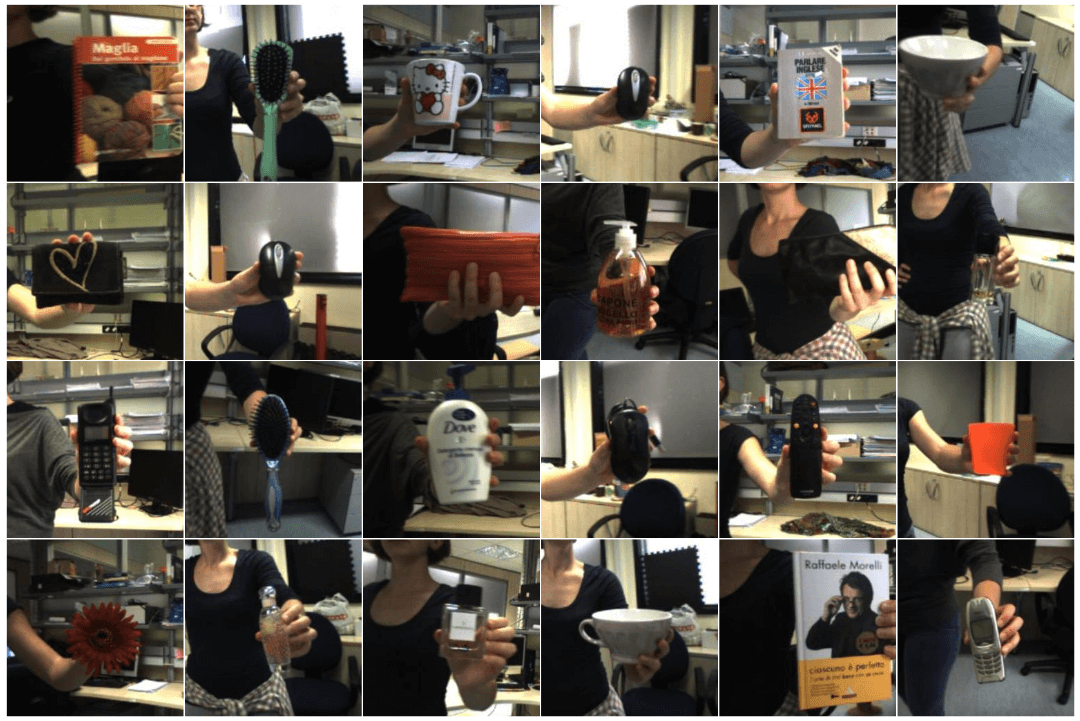
\includegraphics[width=\linewidth]{./img/icw-samples.png}
        \caption{Random sample from the iCubWorld dataset.}\label{fig:icw-samples}
    \end{figure}

    \paragraph{Dataset Statistics}
    For our domain adaptation purposes, we divided the original dataset into two sub-datasets, that we called \textit{Left 1} and
    \textit{Left 2}. These names stem from how we divided the original dataset. In the background change transformation, the human
    moved in a semi-circle around the robot. We put frames at the beginning of the semi-circle in \textit{Left 1}, and frames at the
    end of it in \textit{Left 2}, while we have discarded frames at the center of the circle. Thus we have two DA settings: one in which
    the source is Left 1 and the target is Left 2, and vice-versa. Left 1 has 4500 images, while Left 2 has 3000 images. The classes
    are perfectly balanced, in that each one has the same number of samples.

    \paragraph{Training methodology}
    \paragraph{Testing methodology}
    \paragraph{Results}

\end{document}
